\documentclass{article}
% translate with >> pdflatex -shell-escape <file>

% This file is used as unit test for pgfplots, copyright by Christian Feuersaenger.
% 
% See
%   http://pgfplots.sourceforge.net/pgfplots.pdf
% for pgfplots.
%
% Any required input files (for <plot table> or <plot file> or the table package) can be downloaded
% at
% http://www.ctan.org/tex-archive/graphics/pgf/contrib/pgfplots/doc/latex/
% and
% http://www.ctan.org/tex-archive/graphics/pgf/contrib/pgfplots/doc/latex/plotdata/

\usepackage{pgfplots}
\usepgfplotslibrary{units}
\pgfplotsset{compat=newest}

\pagestyle{empty}

\begin{document}
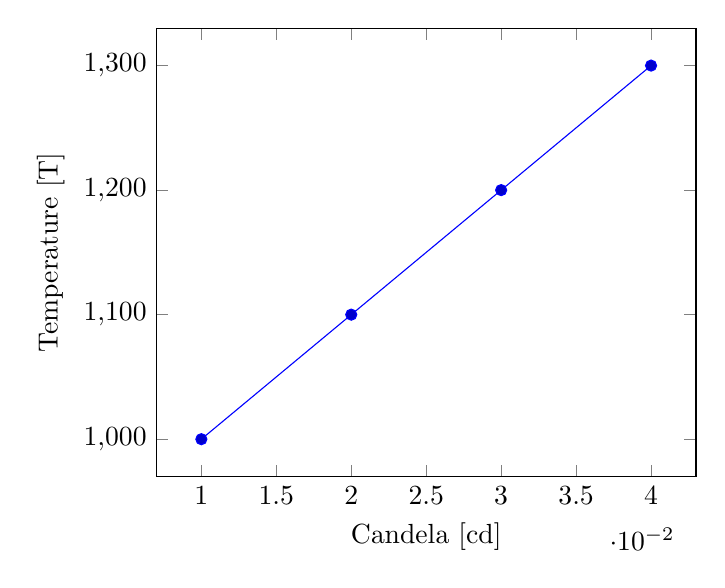
\begin{tikzpicture}
  \begin{axis}[xlabel=test,x unit=cd,xlabel=Candela,y unit=T,ylabel=Temperature]
    \addplot coordinates {
        (0.01,1000)
        (0.02,1100)
        (0.03,1200)
        (0.04,1300)
    };
  \end{axis}
\end{tikzpicture}
\end{document}
